\capitulo{6}{Resultados y conclusiones obtenidas sobre los datos}

\section{Introducción}
En este capítulo se detallan los resultados y conclusiones que se han podido obtener de los datos y de los modelos creados para así poder determinar cuáles son las mejores estrategias de rotación de jugadores y así poder definir conclusiones claras que puedan ayudar a los entrenadores y directivos a tomar decisiones. 

\section{Conclusiones extraídas del análisis previo de los datos}

Previo al entrenamiento de los modelos, se ha realizado un análisis de los datos obtenidos para 
extraer posibles patrones sobre ellos y obtener conclusiones que puedan ayudar a los entrenadores a la hora de la toma de decisiones. Para realizar esto, se ha extraído el valor de cada indicador 
analizado de forma general para cada equipo en el último partido de la temporada que jugase y 
después se ha realizado la clasificación ordenando de mayor a menor por este indicador entre 
todos los equipos de esa liga. Después se ha evaluado en cuantas posiciones difiere la posición de 
este equipo en esta clasificación por el indicador respecto a la clasificación original ordenando 
por puntos. 

Con estos datos, se ha realizado un mapa de calor de manera que las diferencias negativas se 
marcasen en rojo y las diferencias positivas se marcasen en verde. Mediante este análisis se 
pretenden desmentir o confirmar pensamientos que están extendidos de forma generalizada en el 
mundo de fútbol y que pueden ayudar a extraer conclusiones de los datos, como por ejemplo, los 
equipos que hacen más cambios introduciendo delanteros, anotan más goles. A continuación, se detalla un ejemplo de cómo se explica y analiza este mapa de calor.

En la Figura \ref{fig:explicacion-mapa} se muestran los datos para los equipos de LaLiga en la temporada 2024 para 
la proporción de cambios en la alineación de delanteros en sus partidos en general.

\begin{figure}[H]
    \centering
    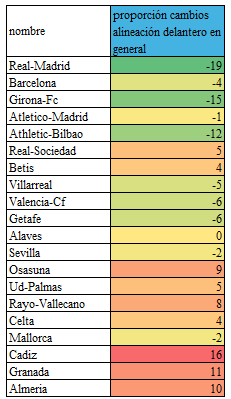
\includegraphics[scale=0.75]{svg/explicacion-tabla.png}
    \caption{Explicación sobre el mapa de calor para las diferencias de posiciones de clasificación. }
    \label{fig:explicacion-mapa}
\end{figure}



Aquí se puede observar que el Real Madrid tiene un valor de -19 en verde. Esto se explica porque 
hay 19 posiciones de diferencia entre su posición por la clasificación por puntos y su posición en 
la clasificación por este indicador que es la proporción de cambios en la alineación de delanteros 
en sus partidos en general. Por lo tanto, es un equipo con alto rendimiento ya que ocupa posiciones 
altas en la clasificación por puntos, pero sin embargo no suele realizar muchos cambios de 
delanteros en sus alineaciones iniciales. Por el contrario, el Cádiz que tiene un valor de 16 en rojo, 
se debe a que ocupa una baja posición en la clasificación por puntos, pero por otro lado, ocupa 
una alta posición en la clasificación por este indicador. Por lo tanto, es un equipo que tiene pocos 
puntos y un bajo rendimiento y que tiene una elevada proporción de cambios de delanteros en su 
alineación inicial.

En conclusión, en el análisis de este indicador se aprecia que los equipos de la zona alta de la 
clasificación por puntos tienen valores bajos en la proporción de cambios de delanteros en la 
alineación inicial y los equipos de la zona baja de la clasificación por puntos tienen valores altos 
en la proporción de cambios de delanteros en la alineación inicial.

A continuación, se detallan el resto de las principales conclusiones extraídas que se han podido 
apreciar de manera generalizada en todas las temporadas de las ligas evaluadas mediante este 
análisis:


\begin{itemize}
    \item Los equipos que realizan más cambios en las alineaciones iniciales entre un partido y otro
    tienden a estar en las posiciones más bajas de la clasificación y por el contrario, los 
    equipos que realizan menos cambios en las alineaciones iniciales entre un partido y otro, 
    tienden a estar en las posiciones más altas de la clasificación. Este efecto se aprecia sobre 
    todo si los cambios en las alineaciones iniciales afectan a los defensas o delanteros.
    \item Los equipos que realizan más cambios antes del descanso tienden a estar en posiciones 
    más bajas en la clasificación. Esto se puede apreciar sobre todo en la Premier League y 
    Bundesliga. Por otro lado, para todas las ligas, los equipos que hacen menos cambios 
    entre los minutos 61 a 75, tienden a ocupar posiciones más altas en la clasificación.
    \item Los equipos que hacen más cambios sacando defensas e introduciendo jugadores más
    ofensivos, suelen ocupar posiciones más bajas en la clasificación. Por otra parte, los 
    equipos que hacen menos cambios sacando delanteros e introduciendo jugadores más
    defensivos, tienden a ocupar posiciones más altas en la clasificación.
    \item Respecto a la media de los minutos en la que los equipos realizan los cambios, los equipos 
    de la zona alta de la clasificación tienen valores más bajos en este valor, por lo tanto, de 
    media suelen realizar los cambios antes.
    \item Los equipos de la zona alta de la clasificación suelen hacer menos cambios de jugadores 
    que han sido amonestados con amarilla.
    \item Finalmente, los equipos de la zona alta de la clasificación suelen tener menores valores en la 
    proporción de cambios que realizan por partido, es decir, en sus partidos no suelen gastar
    los 5 cambios de los que disponen.
    
\end{itemize}

El mapa de calor global agrupando todos los datos de los equipos en las ligas y temporadas consideradas para todos los indicadores analizados se puede ver a continuación en las Figuras \ref{fig:primera-calor}, \ref{fig:segunda-calor} y \ref{fig:tercera-calor}. Sin embargo, es importante detallar los siguientes aspectos sobre estos mapas de calor.
\begin{itemize}
    \item Solo se muestran los datos de las primeras cinco posiciones y de las últimas cinco. En el caso de las últimas cinco se utiliza esa nomenclatura de ultima, penúltima... ya que la Bundesliga tiene menos equipos y por tanto el último de su clasificación ocupa la posición 18 y no la 20 como sucede en LaLiga y la Premier League. Por lo tanto, la última posición, para todas las ligas, se corresponde con el equipo que ocupa la última posición, ya sea la 20 en ligas de 20 equipos (LaLiga y Premier League) o la 18 en la Bundesliga.
    \item Cada valor de este mapa de calor global se calcula mediante el promedio de cada valor en esa posición de los datos de cada liga y temporada analizada. Por lo tanto, los datos que se ven en las Figuras \ref{fig:primera-calor}, \ref{fig:segunda-calor} y \ref{fig:tercera-calor}, se obtienen al hallar el promedio de las diferencias de posiciones para cada una de las diez posiciones que se muestran con los datos de las diferentes ligas y temporadas evaluadas. Por ejemplo, para la primera posición del indicador porcentaje de cambios de defensas a centrocampistas, el valor se ha obtenido calculando el promedio con los valores asociados a la diferencia de clasificación del equipo que acabó en primera posición en la clasificación por puntos en cada una de las temporadas y ligas evaluadas para ese indicador. 
\end{itemize}

\begin{figure}[H]
    \centering
    \rotatebox{90}{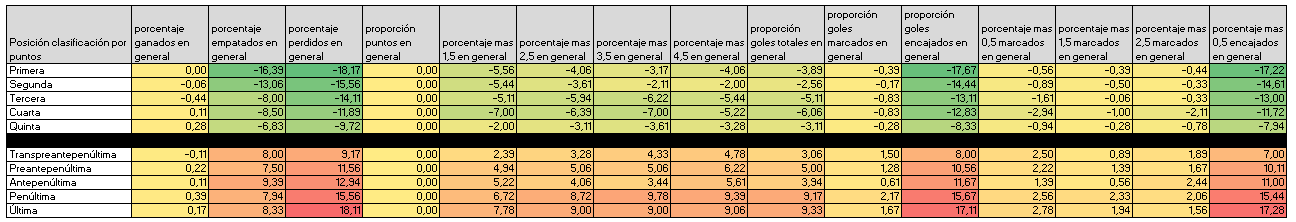
\includegraphics[scale=0.60]{svg/mapa-calor1.png}}
    \caption{Primera parte del mapa de calor global con las diferencias de posiciones de clasificación. }
    \label{fig:primera-calor}
\end{figure}

\begin{figure}[H]
    \centering
    \rotatebox{90}{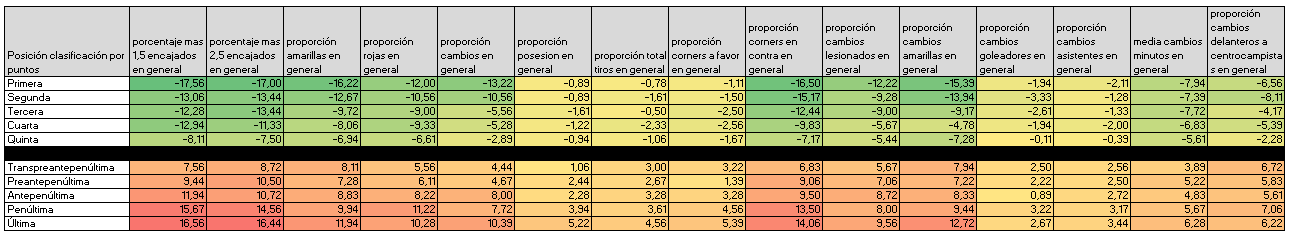
\includegraphics[scale=0.60]{svg/mapa-calor2.png}}
    \caption{Segunda parte del mapa de calor global con las diferencias de posiciones de clasificación. }
    \label{fig:segunda-calor}
\end{figure}

\begin{figure}[H]
    \centering
    \rotatebox{90}{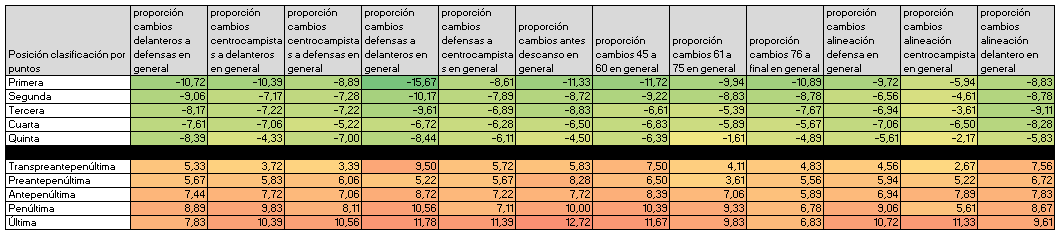
\includegraphics[scale=0.60]{svg/mapa-calor3.png}}
    \caption{Tercera parte del mapa de calor global con las diferencias de posiciones de clasificación. }
    \label{fig:tercera-calor}
\end{figure}












\section{Conclusiones extraídas al entrenar los modelos}




Se ha podido observar que en las predicciones realizadas por el modelo para predecir el ganador 
del partido, las variables que más repercusión tienen para aumentar la probabilidad de victoria del
equipo local son la proporción de este equipo de realizar cambios entre los minutos 61 a 75, la
proporción de cambios de defensas a centrocampistas y la proporción de cambios de
centrocampistas a defensas y para el visitante la proporción de este equipo de cambios de
centrocampistas a defensas, la proporción de cambios de defensas a delanteros y la proporción de 
cambios entre el minuto 76 al final. Los equipos con valores más elevados en estos indicadores 
tienen según el modelo más probabilidad de ganar el partido.

Por otro lado, para el modelo que predice la probabilidad que tiene el equipo local de marcar un 
determinado número de goles, las variables que tienen más repercusión para aumentar las 
probabilidades de que el equipo marque más goles son la proporción de este equipo de cambios 
entre los minutos del 45 al 60, la proporción de cambios de defensas a centrocampistas, la 
proporción de cambios de defensas a delanteros y la proporción de cambios de centrocampistas a 
delanteros. Los equipos locales con valores más elevados en estos indicadores tienen según este 
modelo más probabilidades de anotar un número más elevado de goles.

Para el modelo que predice la probabilidad que tiene el equipo visitante de marcar un determinado
número de goles, las variables que más repercusión tienen para aumentar las probabilidades de 
que el equipo marque más goles son la proporción del equipo de cambios de delanteros en la 
alineación inicial, la proporción de cambios de centrocampistas en la alineación inicial, la 
proporción de cambios de defensas a centrocampistas y la proporción de cambios entre los 
minutos 76 al final. Los equipos visitantes con valores más elevados en estos indicadores tienen 
según este modelo más probabilidades de anotar un número más elevado de goles.

\section{Conclusiones y resultados generales}


Previo a los modelos, el análisis previo de los datos ha revelado diferentes patrones que pueden 
ayudar enormemente a los entrenadores a tomar decisiones sobre los jugadores para aumentar el 
rendimiento del equipo, como evitar realizar muchos cambios en las alineaciones iniciales o evitar 
realizar muchos cambios antes del descanso, ya que ambos factores en este caso están 
estrechamente relacionados con los equipos de la zona baja de la clasificación. 

Por otro lado, realizar menos cambios en las alineaciones iniciales y menos cambios entre los 
minutos 61 y 75 se asocia a equipos que ocupan las posiciones más altas de la clasificación, y esto 
puede ser una buena señal de que estas estrategias ayudan al buen rendimiento del equipo.
En cuanto a las posiciones de los jugadores que son afectados por los cambios, realizar cambios 
ofensivos quitando defensas es una estrategia que se puede apreciar sobre todo en los equipos de 
la zona baja de la clasificación y por lo tanto no ayuda a su rendimiento. Por otra parte, realizar 
pocos cambios sacando delanteros e introduciendo jugadores más defensivos es una estrategia 
utilizada por los equipos de la zona alta de la clasificación y por lo tanto parece que contribuye a 
su éxito y buen rendimiento.

Sobre los minutos en los que se realizan los cambios, los equipos que de media realizan los 
cambios antes suelen estar en la zona alta de la clasificación y lo mismo es aplicable a los cambios 
que reemplazan jugadores amonestados con amarilla ya que los equipos con menos cambios de 
este tipo ocupan posiciones más altas.

Finalmente, otro dato bastante significativo y curioso es que los equipos de la zona alta de la 
clasificación tienen valores más bajos en el número de cambios por partido que hacen, es decir, 
no gastan todos los cambios de los que disponen. Esto puede contradecir la creencia generalizada 
de que al realizar más cambios el equipo debería de rendir más porque introduce jugadores 
totalmente frescos pero parece que, este análisis muestra lo contrario, que conviene mantener los 
jugadores que estén en el campo y no necesariamente gastar todos los cambios de los que 
disponen.
